
\chapter{Rendering} \label{rendering}

Our landscape rendering system consists of three primary components - a nearby terrain renderer, a distant terrain renderer, and a forest renderer.
The nearby terrain renderer uses a meshing algorithm influenced by voxel terrain systems (Section \ref{voxterrain}).
This mesh generation is expensive but is necessary for meaningful player interaction and is limited to a very narrow region around the viewpoint.
Far terrain is rendered using a modified implementation of geometry clipmaps (Section \ref{clipterrain}).
The nature of the clipmaps algorithm makes it possible to extend the terrain view distance substantially with minimal overhead.
Our forest system uses mesh instances, impostors, and a similar representation called facades to render vast forests (Section \ref{forests}).
The system is designed to render a large number of individual trees with the highest performance possible.
In addition to these three primary components, our system also renders water and other additional environment aspects, discussed in Sections \ref{sec:water} and \ref{sec:env}.

\section{Nearby Terrain} \label{voxterrain} %%%%%%%%%%%%%%%%%%%%%%%%%%%%%%%%%%%%%%%%%%%%%%%%%%%%%%%%%%%%%%%%%%%%%%%%%%%%%%%%%%%%%%%%%%%%%%%%%%%%%%%%%%%%%%%%%%%%%%%%%%%%%%%%%%%%%%

Nearby terrain is rendered using a pseudo-voxel representation designed to allow for sloped surfaces while maintaining intuitive live editing capabilities.
A voxel algorithm that uses uniform voxel size is simple to implement and manage but is poorly suited to represent sloped surfaces.
Fully volumetric terrain implementations allow for arbitrary slopes but are less intuitive for manipulation by players and navigation by AI.
We utilize a pseudo-voxel system that allows for diagonal faces in addition to solid voxels.
This system allows for simple grid-based editing and simple physics calculations, while allowing sloped polygonal faces that are more aesthetically pleasing than simple voxels.

\subsection{Voxel algorithm}

In principle, the system works by breaking down each individual voxel into eight sub-voxels (one for each corner of the cube) and generating diagonal faces based on which of these sub-voxels are occupied.
However, certain sub-voxel configurations are considered degenerate and are automatically trimmed to a lesser configuration.
For example, in our system any pseudo-voxel with only a single sub-voxel occupied is automatically trimmed to an empty voxel.
In this case the trimming occurs because there is no diagonal face to represent just a single corner of a voxel.
Figure \ref{fig:minimumvoxel} shows the pseudo-voxel with the fewest possible sub-voxels, four.

\begin{figure}
	\centering
		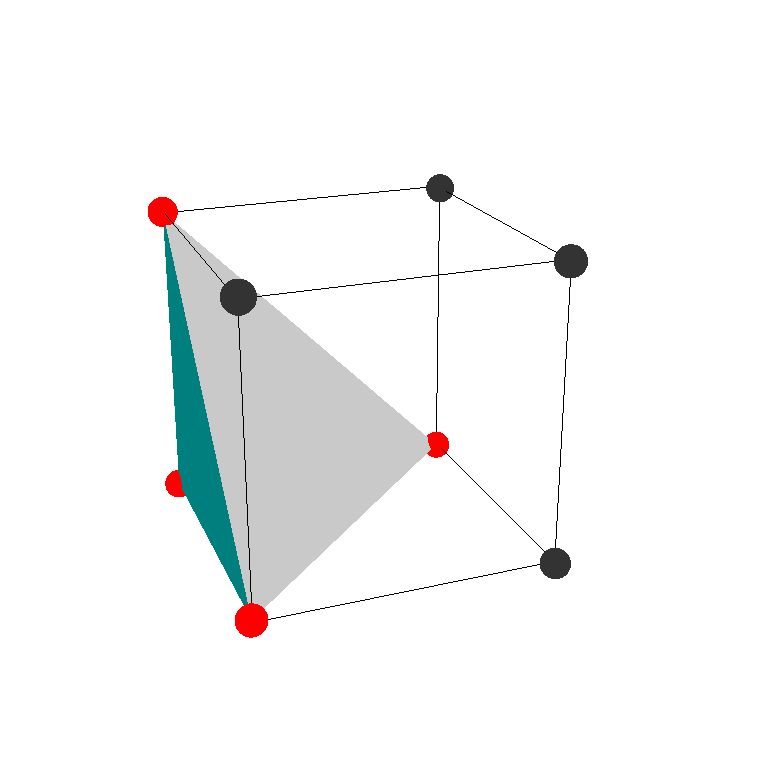
\includegraphics[width=0.5\textwidth]{figures/minimumvoxel_edges.png}
	\caption{Red spheres indicate a full sub-voxel, grey indicates an empty sub-voxel.}
	\label{fig:minimumvoxel}
\end{figure}

The system can therefore trivially trim any pseudo-voxel configuration with fewer than four sub-voxels.

The system also trims certain pseudo-voxel configurations to a simpler configuration.
See Figure \ref{fig:voxelrejected} for an example.

\begin{figure}
	\centering
		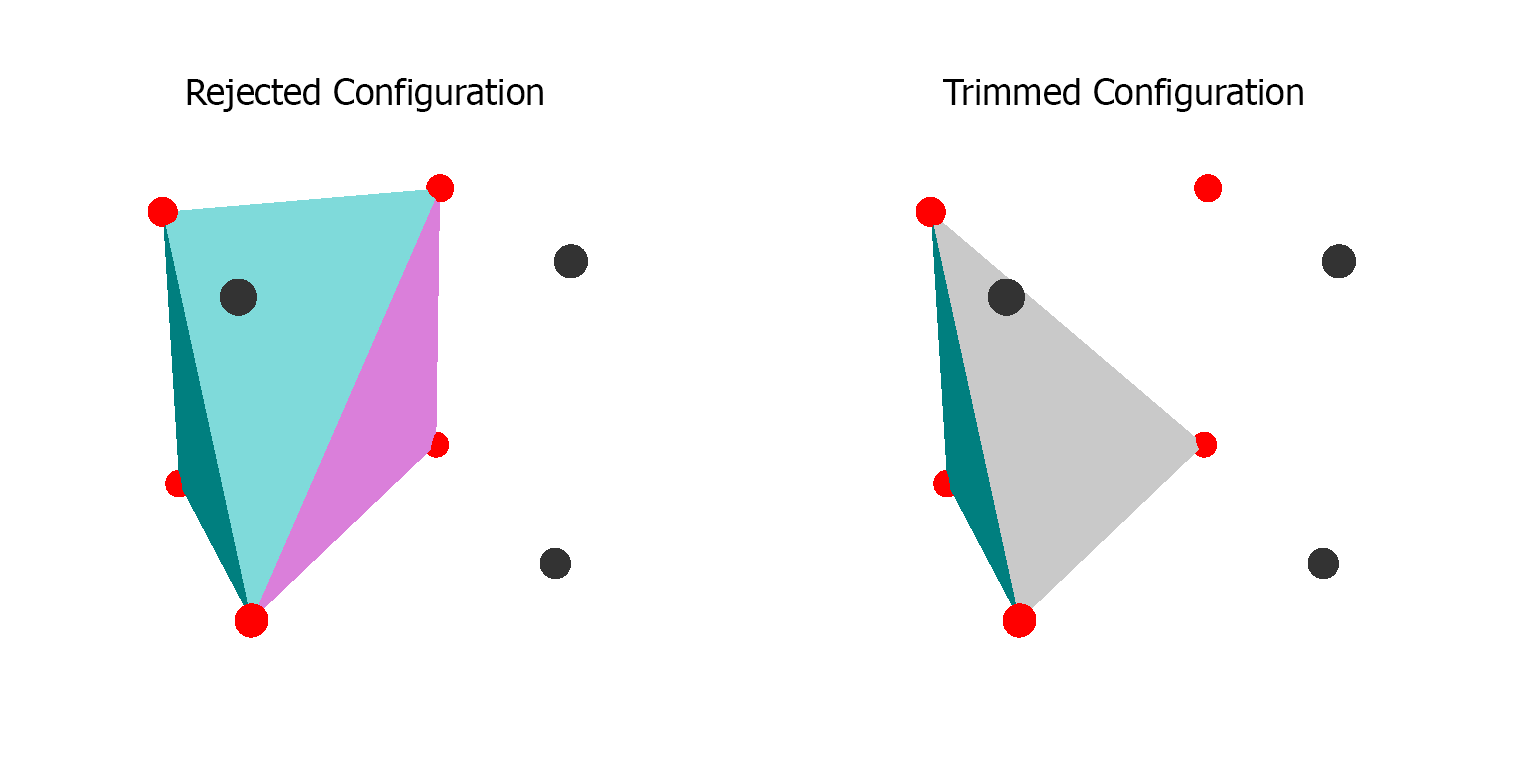
\includegraphics[width=1.0\textwidth]{figures/voxelrejected.png}
	\caption{
		Red spheres indicate a full sub-voxel, grey indicates an empty sub-voxel.
		The image on the left shows a possible triangulation for this sub-voxel configuration.
		However, our algorithm rejects this configuration and instead generates the triangulation on the right.
	}
	\label{fig:voxelrejected}
\end{figure}

This trimming is performed to preserve smooth slopes of generated terrain.
See Figures \ref{fig:trimcomparison1} and \ref{fig:trimcomparison2} for a comparison between untrimmed and trimmed sub-voxel configurations.

\begin{figure}
	\centering
		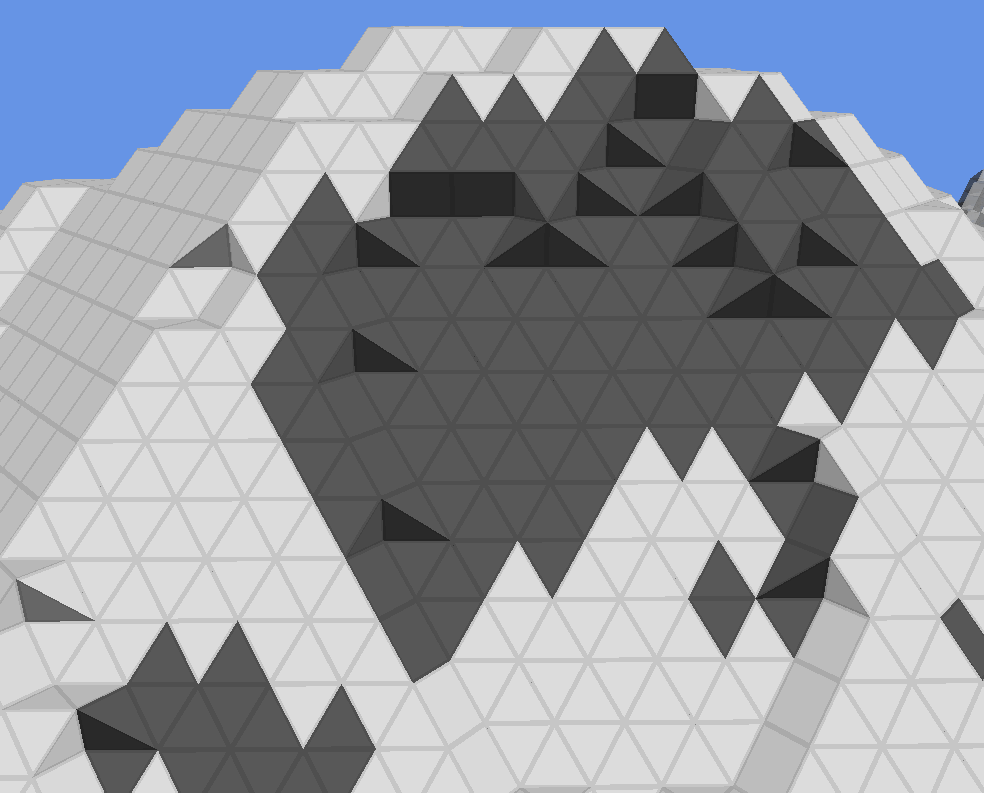
\includegraphics[width=0.75\textwidth]{figures/trimcomparison1.png}
	\caption{
		Voxel triangulation of a mountaintop without sub-voxel trimming enabled.
	}
	\label{fig:trimcomparison1}
\end{figure}

\begin{figure}
	\centering
		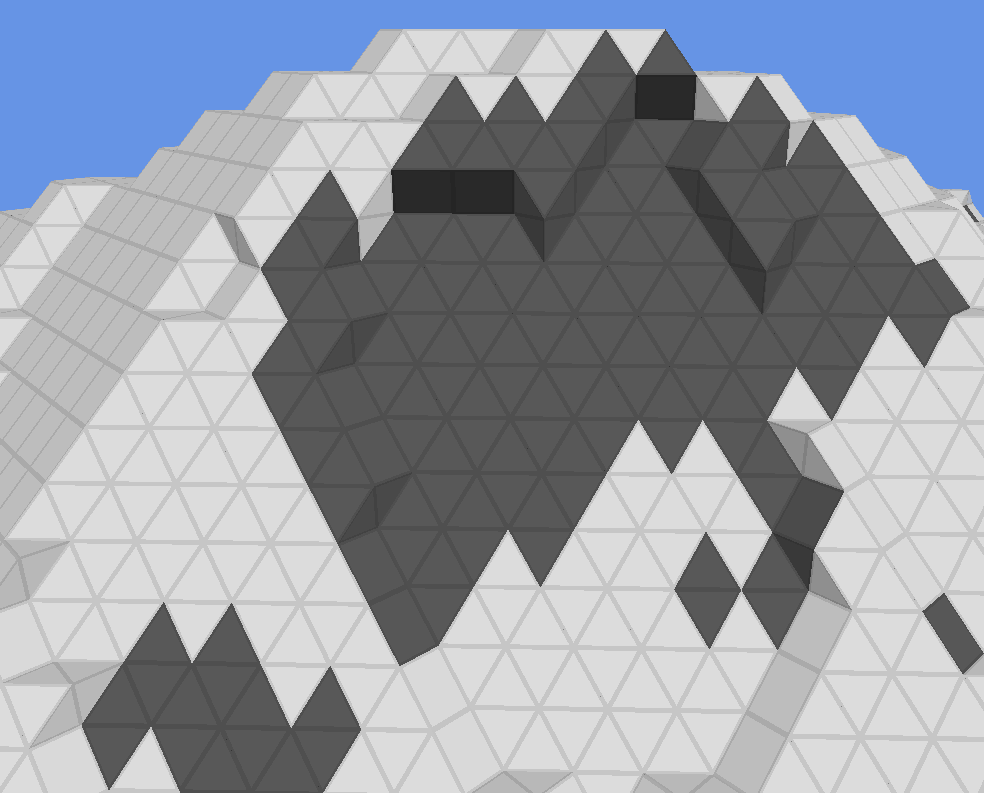
\includegraphics[width=0.75\textwidth]{figures/trimcomparison2.png}
	\caption{
		Voxel triangulation of a mountaintop with sub-voxel trimming enabled.
	}
	\label{fig:trimcomparison2}
\end{figure}

\subsection{Face Generation}

Triangles are generated for each pseudo-voxel configuration using lookup tables for efficiency and simplicity.
The largest lookup table is 12 kilobytes, so the memory impact of using the lookup tables is minimal.
Triangles are divided into two categories: interior and exterior.

\subsubsection{Exterior Faces}

Exterior triangles are the triangles that would normally be generated by a simple voxel system - the faces of a cube.
Exterior triangles are checked against each neighboring pseudo-voxel for visibility.
In the trivial case, a completely solid voxel surrounded entirely by solid voxels produces no triangles, since all exterior triangles are occluded by the exterior faces of each neighboring voxel.

\subsubsection{Interior faces}

Interior faces are the triangles that are unique to Relic's voxel system, as opposed to an ordinary voxel system that only generates exterior faces.
Interior faces have some form of diagonal slope see Figure \ref{fig:interiorfaces2} for a demonstration of each type of interior triangle that Relic generates.

\begin{figure}
	\centering
		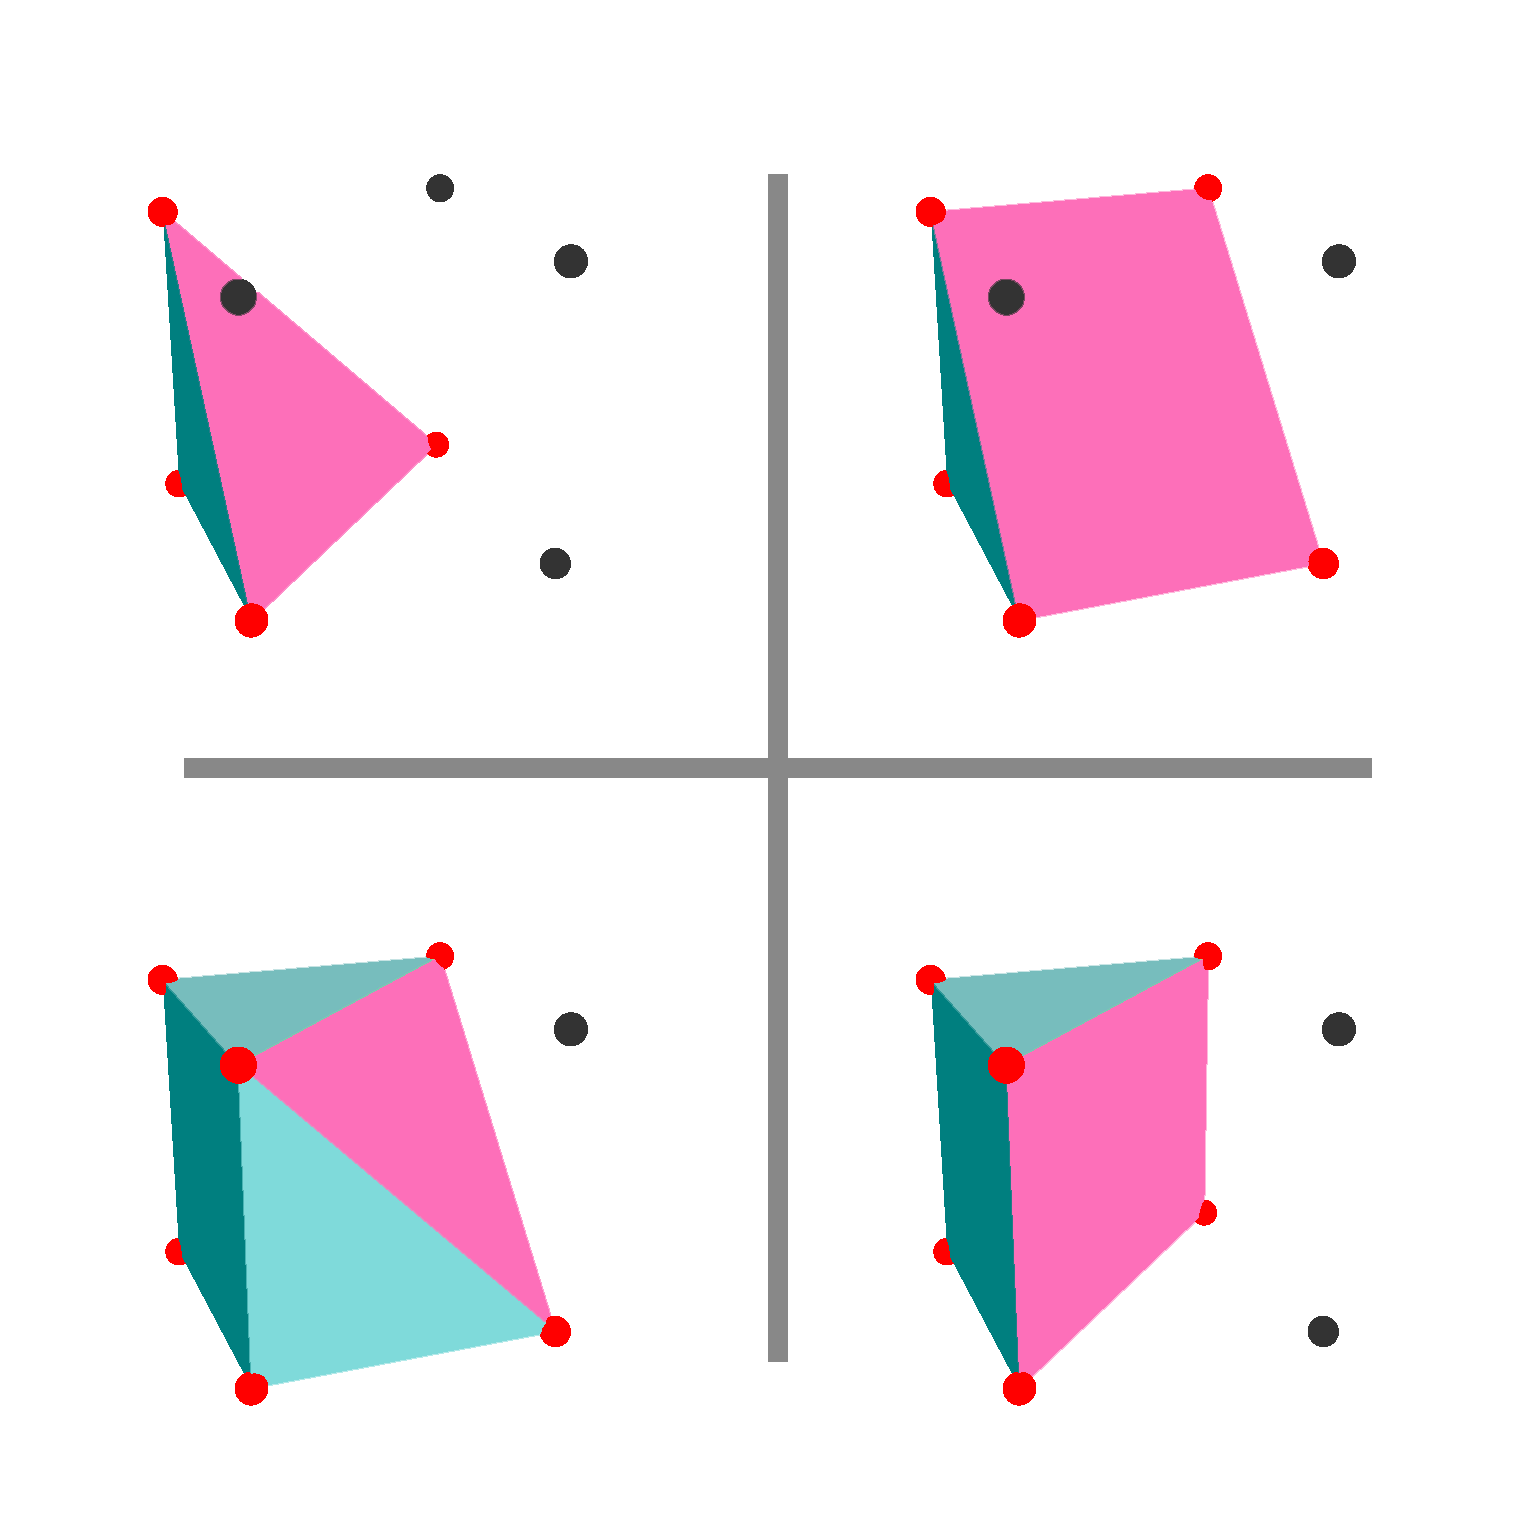
\includegraphics[width=0.75\textwidth]{figures/interiorfaces2.png}
	\caption{
		Example of the four types of interior face.
		Each pink face is an interior face.
		Note that this is just one possible orientation of each class of interior face, but each class can be oriented in either four or eight directions.
		(The left two classes have eight orientations and the right two have four).
	}
	\label{fig:interiorfaces2}
\end{figure}

\subsection{Rendering}

The world is divided into chunks for triangulation and rendering purposes.
Each chunk is a 16x16x16 volume of voxels.
Relic generates voxels at a resolution of one voxel per foot, so each chunk is also 16x16x16 feet in dimension.

One triangle mesh is generated per chunk.
Each chunk tracks its neighbors in all six face directions so that occluded exterior faces can always be accurately detected.
This means that a ring of non-visible chunks must be loaded around all visible chunks, since no visible chunk can have an unloaded neighbor.

In order to determine which chunks are visible, a large sphere is placed around the camera and any chunk that intersects this sphere is loaded and rendered.
As the camera moves, chunks that leave this sphere are unloaded and chunks that enter it are loaded.

Screen-space ambient occlusion is used to help visual understanding of the voxel terrain shape.


\section{Far Terrain} \label{clipterrain} %%%%%%%%%%%%%%%%%%%%%%%%%%%%%%%%%%%%%%%%%%%%%%%%%%%%%%%%%%%%%%%%%%%%%%%%%%%%%%%%%%%%%%%%%%%%%%%%%%%%%%%%%%%%%%%%%%%%%%%%%%%%%%%%%%%%%%%%%%%%%%%%%%%%%%%%%%%%%

The voxel terrain described in the previous section is ideal for editability and representation of features such as overhangs and caves, but it is very expensive to both generate and render.
In order to maximize the view distance of the Relic world, far terrain is rendered using a flat-shaded implementation of geometry clipmaps with a few modifications.

\subsection{Pre-calculated Index Buffer}

The original geometry clipmaps implementation recalculates index buffers pre-frame so that each layer can grow and expand organically.
This makes it possible to seamlessly transition to lower-resolution terrain when the viewpoint moves rapidly.

However, our system locks the size of each layer so that the index buffers can be pre-calculated.
This was found to significantly reduce CPU overhead.
This means that while the original geometry clipmaps algorithm would simply show less high-frequency detail when the viewpoint moves rapidly, our system slows down with increased load times when the viewpoint moves rapidly.
However, our clipmaps implementation is part of an engine designed for a game, where player movement speed will inherently be limited by a physics simulation.
In addition, rapid movement of the viewpoint will require all other systems (voxel terrain, forests, physics, etc.) to stop and load new data.
As such, allowing the geometry clipmaps algorithm to continue running in this scenario would not be helpful.

\subsection{Normal Calculation}

Since our terrain is flat-shaded for a polygonal effect, the per-quad normals provided by a normal map must be inaccurately applied to two triangles.
We also found that normal calculation from our procedural generation system incurred significant CPU overhead.
Accurate normal calculation in transition regions was also difficult.

Our implementation uses a per-triangle normal calculation in a geometry shader so that accurate normals are always calculated for each triangle.
This saves significant CPU time as normals don't need to be pre-calculated or sent to the GPU normal map.
The addition of the geometry shader was found to not have a significant decrease in rendering performance.

\subsection{Terrain Blending}

In order to use both the near and far terrain representations, Relic implements a blend region between the two systems.
This blend is implemented in a post-processing pass that uses separate frame buffers for each terrain representation.
The algorithm operates on individual fragments.
If both systems are visible at a given fragment, and the distance to the fragment is near the maximum distance of the near terrain representation, a blend of the two systems is used.
For all other fragments, the near terrain fragment is selected if it is visible, otherwise the far terrain fragment is selected.
However, if only the far terrain fragment is visible but the distance is closer to the viewpoint than the start of the blend region, the fragment is discarded.
This is to prevent visual artifacts when the far terrain representation happens to be higher on the Y axis than the near representation.
See Figure \ref{fig:terrain_overlap} for an example of where this artifact may occur.

\begin{figure}
	\centering
		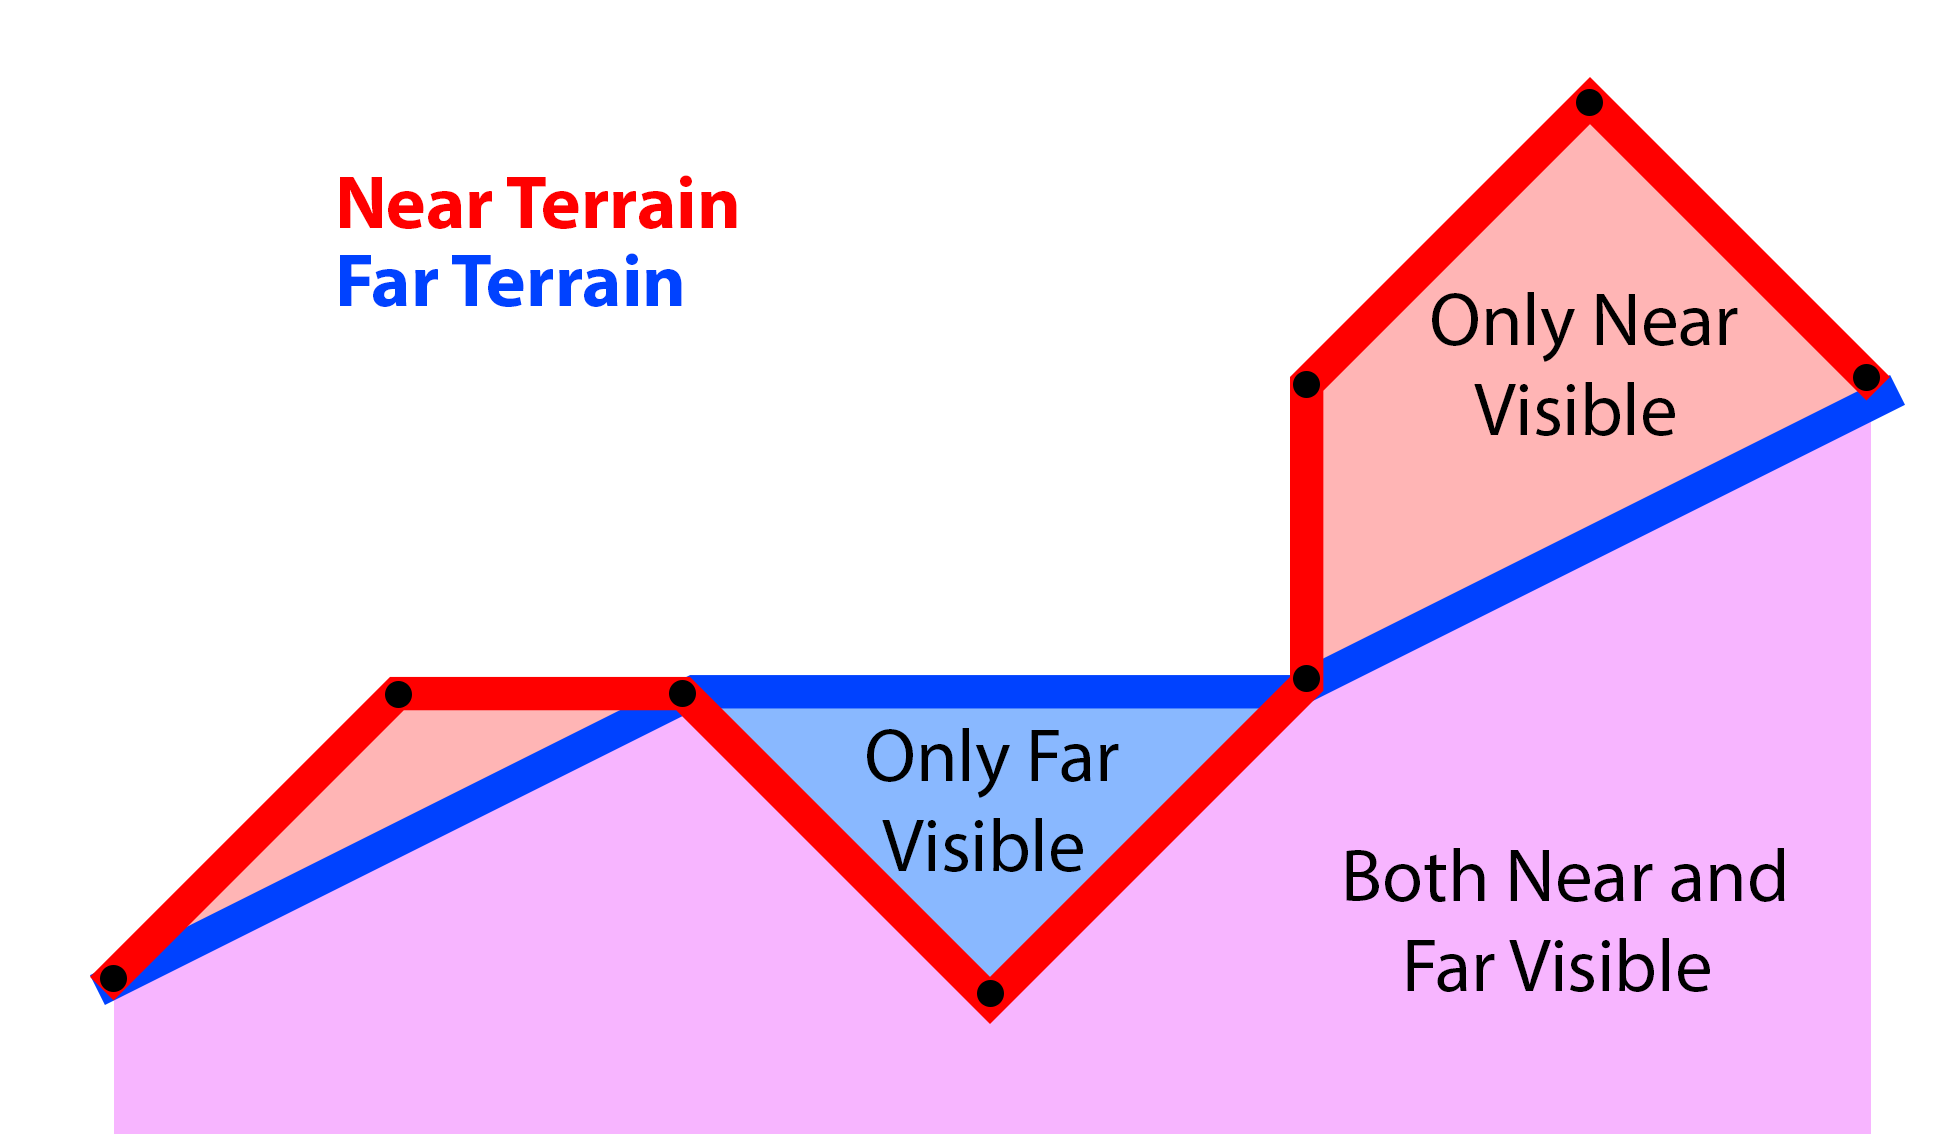
\includegraphics[width=0.75\textwidth]{figures/terrain_overlap.png}
	\caption{
		In this image the red line represents the shape of the near (voxel) terrain and the blue line represents the shape of the far (clipmaps) terrain.
		The light blue shaded region is an area where the far terrain might show above the near terrain from this side view.
		Relic solves this problem by culling all nearby fragments from the far terrain render.
	}
	\label{fig:terrain_overlap}
\end{figure}


\section{Forests} \label{forests} %%%%%%%%%%%%%%%%%%%%%%%%%%%%%%%%%%%%%%%%%%%%%%%%%%%%%%%%%%%%%%%%%%%%%%%%%%%%%%%%%%%%%%%%%%%%%%%%%%%%%%%%%%%%%%%%%%%%%%%%%%%%%%%%%%%%%%%%%%%%%%%%%%%%%%%%%%%%%%

Our vegetation system currently supports rendering a large number of low-poly spruce trees, but could be expanded to support other types of vegetation.
The system uses three levels of detail: mesh instances, impostors, and mesh facades.

Trees are rendered in groups similar to the chunk system used by nearby terrain.
Mesh instances and impostors render many trees per group, whereas the mesh facade renders a single mesh to represent each group.

\subsection{Mesh Instances}

The mesh instances layer simply uses instance rendering to draw the tree model in several places.

\subsection{Impostors}

The impostors layer draws a billboard for each tree in the group.
During initialization, the colors and normals of the tree model are rendered to textures for use in drawing each impostor.
The impostors are locked in their X and Z axis rotation so that the base of the impostor always rests on the ground, and to reduce artifacts when the camera is high above or below the impostor.
See Figure \ref{fig:tree_billboards} for a comparison between the cylindrical billboards we use and the alternative spherical billboard.
The rotation around the Y-axis is used to rotate the normals of the impostor so that lighting is accurate for impostors in all directions.

\begin{figure}
	\centering
		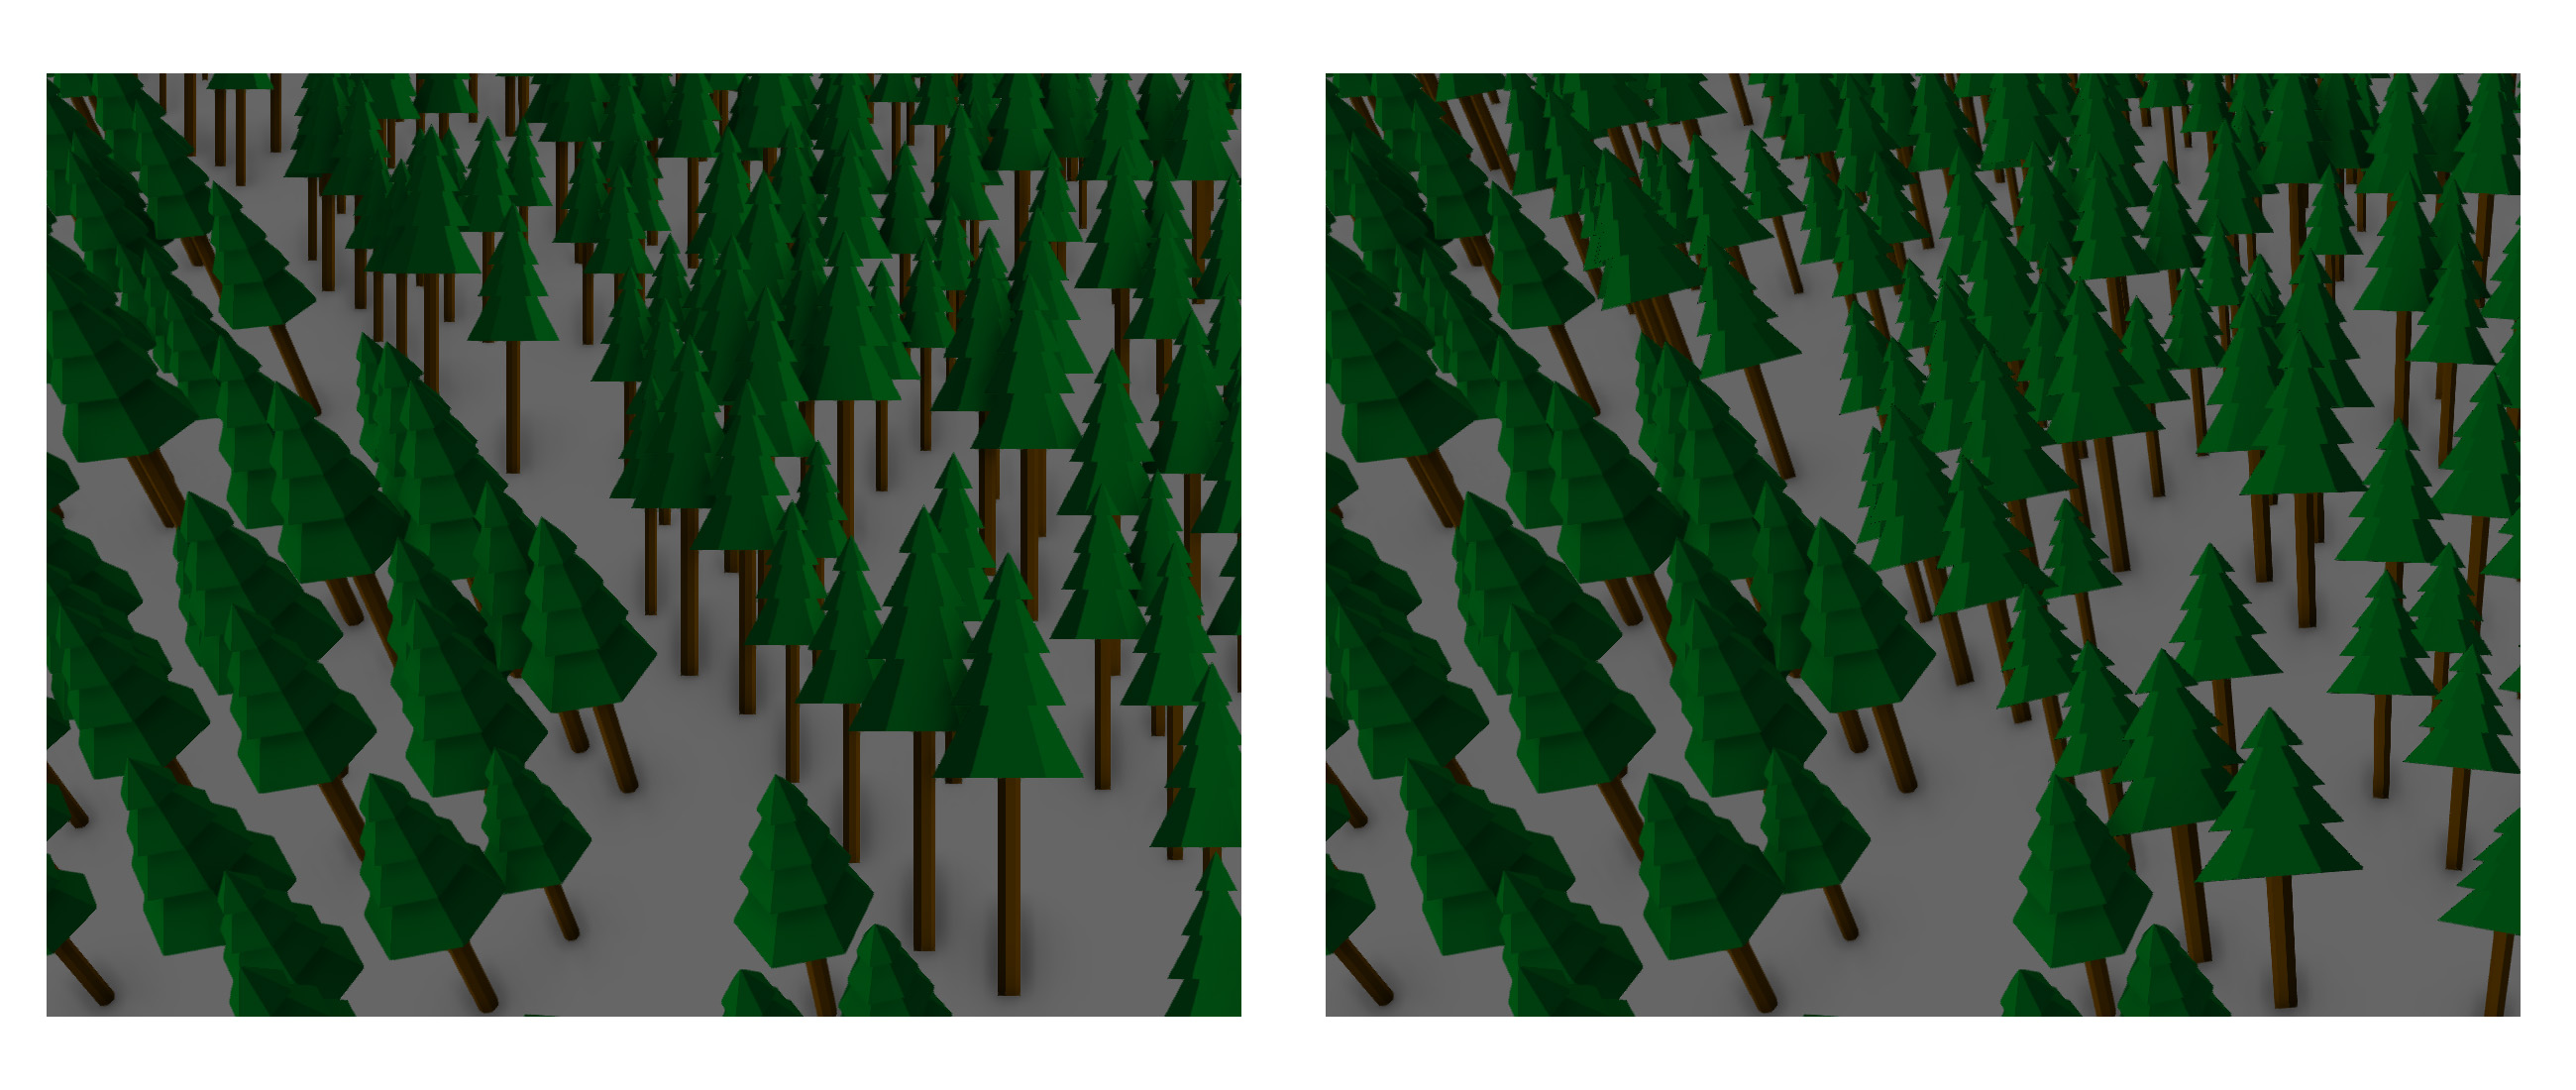
\includegraphics[width=1.0\textwidth]{figures/tree_billboards.jpg}
	\caption{
		In the left image, tree impostors are rendered on spherical billboards.
		At this elevated viewpoint, the billboard effect is clearly visible when compared to the tree mesh instances in the lower left corner of the image.
		The right image shows the same scene as rendered by the Relic engine, using cylindrical billboards (where only the Y axis rotates).
	}
	\label{fig:tree_billboards}
\end{figure}

\subsection{Mesh Facades}

The final layer uses a simple mesh to represent a group of trees.
The appearance of this mesh is quite simplistic but at large view distances it is sufficient to represent a group of trees.
See Figure \ref{fig:tree_facades} for a comparison between mesh facades up close and at a distance.

\begin{figure}
	\centering
		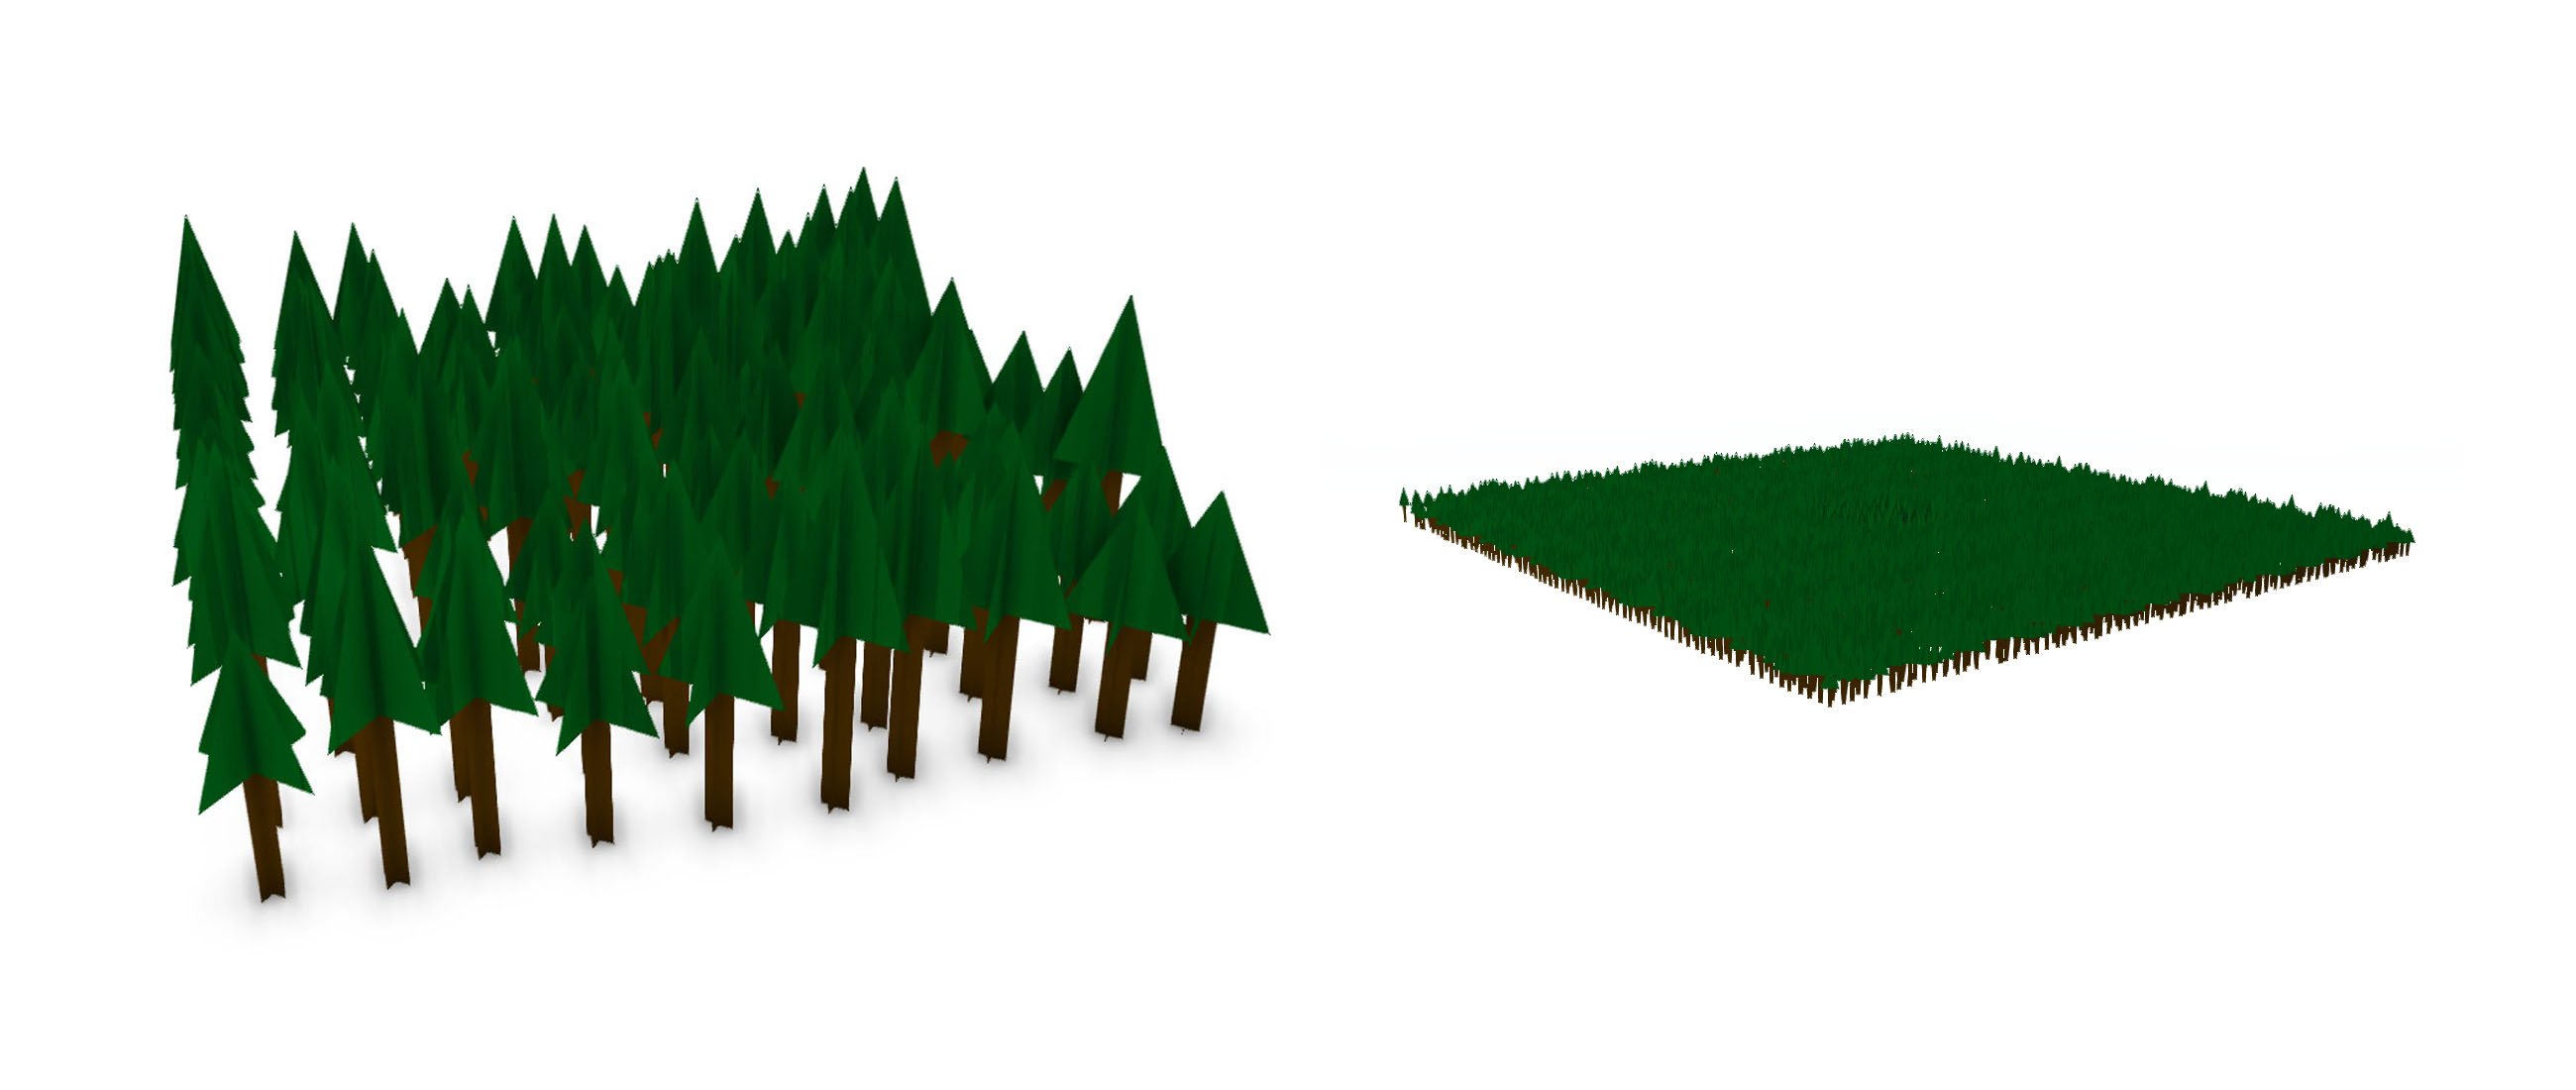
\includegraphics[width=1.0\textwidth]{figures/tree_facades.jpg}
	\caption{
		On the left, a tree facade is shown in detail.
		The image on the right is many tree facades at great distance.
	}
	\label{fig:tree_facades}
\end{figure}

\section{Water} \label{sec:water} %%%%%%%%%%%%%%%%%%%%%%%%%%%%%%%%%%%%%%%%%%%%%%%%%%%%%%%%%%%%%%%%%%%%%%%%%%%%%%%%%%%%%%%%%%%%%%%%%%%%%%%%%%%%%%%%%%%%%%%%%%%%%%%%%%%%%%%%%%%%%%%%%%%%%%%%%%%%%%%%%%%


Our water system uses the geometry of our far terrain (geometry clipmaps) implementation for simplicity.

Instead of offsetting each vertex by a heightmap value, however, we used summed Gerstner waves in the vertex shader.
This provides both a vertical offset and a normal to use for rendering.

The result is expensive, but simple and looks reasonable.


\section{Environment} \label{sec:env} %%%%%%%%%%%%%%%%%%%%%%%%%%%%%%%%%%%%%%%%%%%%%%%%%%%%%%%%%%%%%%%%%%%%%%%%%%%%%%%%%%%%%%%%%%%%%%%%%%%%%%%%%%%%%%%%%%%%%%%%%%%%%%%%%%%%%%%%%%%%%%%%%%%%%%%%%%%%%

The system renders a billboard to represent the sun and a sky sphere with vertex colors to represent the sky.

Lighting for all other objects in the scene uses three directional lights: one for direct sunlight, one for scene reflection of sunlight, and one for sky light.
The sunlight has high bright white color and points from the sun position towards the scene.
The scene reflection light has dim white color and points in the opposite direction of the sunlight, with the Y component clamped to zero.
The sky light points directly downward (negative Y) and has soft blue color.

Our system also implements a simple atmospheric scattering simulation by applying fog to each rendered fragment based on scene depth.
The fog color interpolates between dark blue for near fragments and the sky color for far fragments.


\section{Depth Buffer Precision} \label{sec:prec} %%%%%%%%%%%%%%%%%%%%%%%%%%%%%%%%%%%%%%%%%%%%%%%%%%%%%%%%%%%%%%%%%%%%%%%%%%%%%%%%%%%%%%%%%%%%%%%%%%%%%%%%%%%%%%%%%%%%%%%%%%%%%%%%%%%%%%%%%%%%%%%%%%%%%%%%%%%%%

Our system supports very large view distances.
Setting the far plane at sufficient distance for our scene significantly degrades the performance of the depth buffer, even with 32 bits of precision.
Insufficient precision in the depth buffer results in Z-fighting on distant elements and especially noise in the ambient occlusion effect.

\begin{figure}
	\centering
		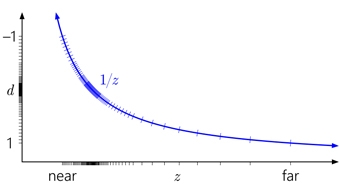
\includegraphics[width=0.6\textwidth]{figures/nvidia_precision_1.jpg}
	\caption{Mapping of Z values to depth values \cite{nvidia_depth_precision}. The tick marks on the blue line indicate the precision of the depth buffer.}
	\label{fig:nvidia_precision_1}
\end{figure}

One problem is that the mapping of Z values to depth values has a reciprocal shape, such that most of the depth buffer precision is alloted for nearby fragments (See Figure \ref{fig:nvidia_precision_1}).
To improve depth buffer performance for far distances, we use the inverted depth buffer trick \cite{nvidia_depth_precision}.
By using a DirectX compatibility feature of OpenGL, we can use a depth buffer ranging from zero to one instead of negative one to one.
Then, by storing depths reversed from the conventional direction, we can utilize the inherent distribution of floating point precision to even out the distribution of depth values in our scene.
The conventional depth direction has near values at zero and far values at one.
However, floating point precision is higher for values closer to zero.
By storing near depths at one and far depths at zero, the additional floating point precision creates a pseudo-logarithmic distribution of depth values.

This results in a significant reduction in depth precision artifacts.
